\autsection{General Approach}{Nelián Colón}

At first, the team will be developing different parts of
the system as they are all loosely coupled. Test driven development will be
done, meaning that after each part gets successfully developed and unit tested,
only then they are integrated and tested from a bigger perspective. The project
is divided into 4 major parts, these are: front end client, back end server,
test framework, and repository manager, as shown in Figure~\ref{arqu}. The team
will be using a single cloud hosted Git repository (GitHub) where the project's
code will live, and will follow best revision control practices. Moreover, the
team will follow the Scrum agile development process.

\begin{figure}[H]
	\centering
	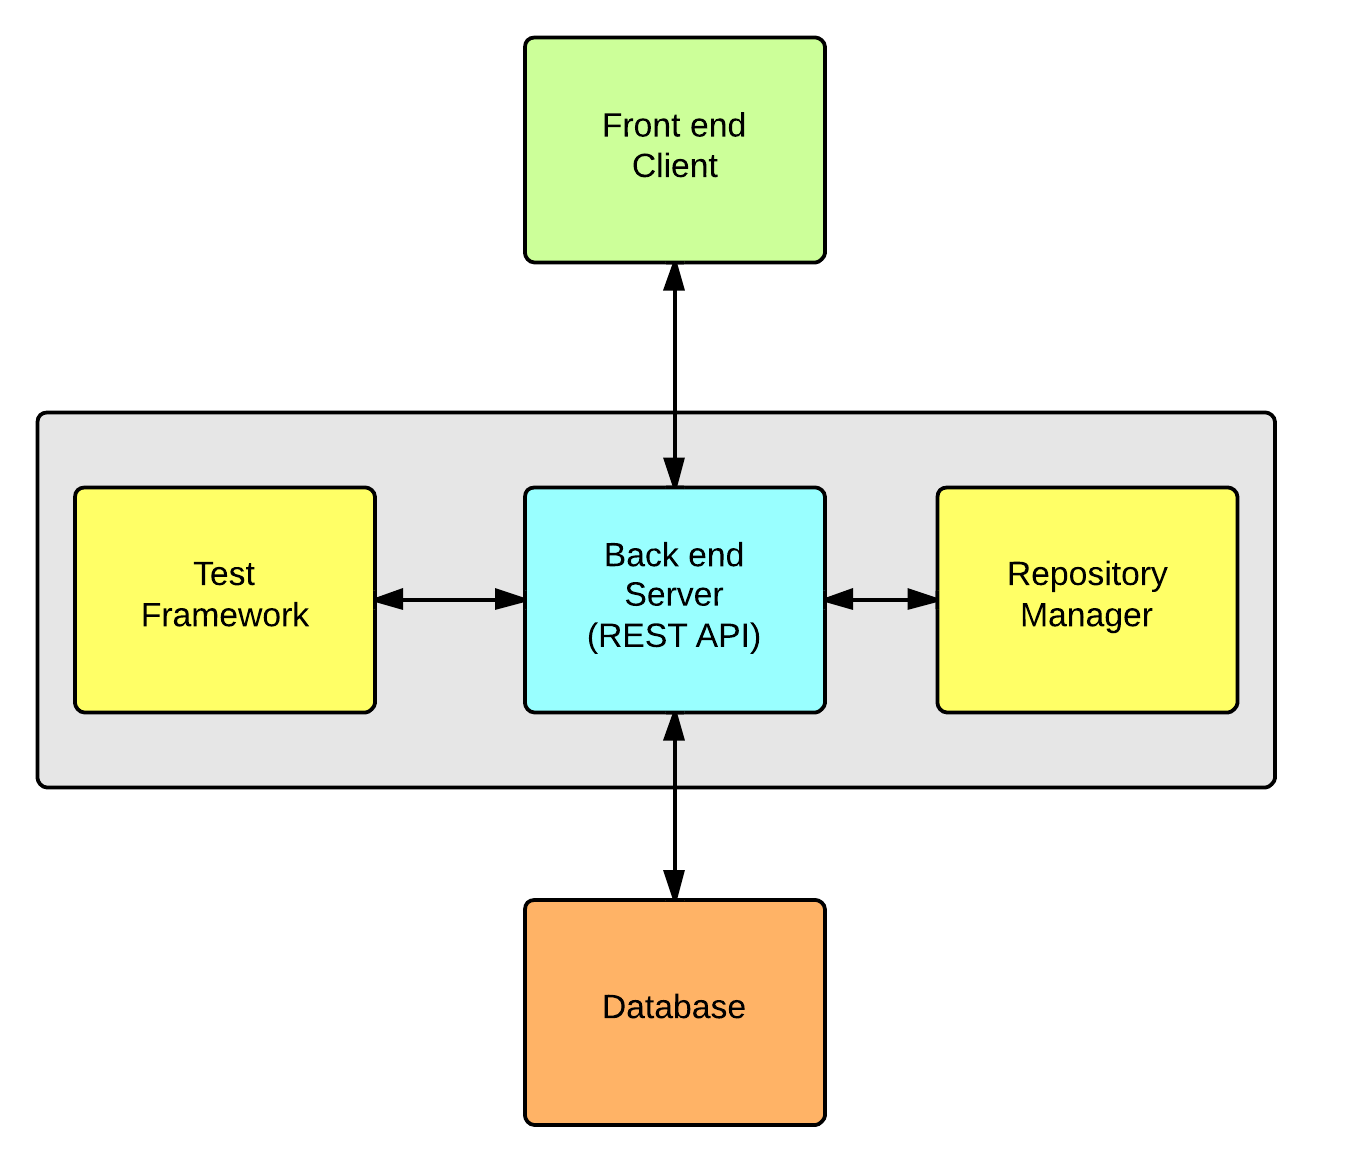
\includegraphics[scale=0.2]{img/bigArquitectOverview}
	\caption{General overview of the system\label{arqu}}
\end{figure}

\subsection{Team Management}

As mentioned before, the team will follow the Scrum agile development process.
Meetings will be held at the start and end of each sprint, these meeting are
sprint planning and sprint retrospective. Each task will have a leader and an
assistant. The leader of each task is completely responsible for the task and
the assistant will assist whenever the leader gets stuck on a problem. Tasks
will have a weight that is going to be decided during the sprint planning
meeting. Table~\ref{tasks} contains the main tasks distribution for the project.
For a more detailed list of task distribution see the Gantt Chart included as a
separate file.

\begin{center}
\setlength{\extrarowheight}{1.5pt}
  \begin{longtable}{|m{3.25in}|c|c|c|}
 \caption{Task Distribution \label{tasks}} \\
   \hline
  
  \centering Task Title & Nelián & Samuel & Daniel \\
  \hline \hline \endfirsthead
  
     \hline

	\centering Task Title & Nelián & Samuel & Daniel \\  
	\hline \hline \endhead
  
  \endfoot  
  
  Project Management and Team Organization & Lead & Assist & \\ \hline
  Web Front end & & Lead & Assist \\ \hline
  Back end Server & & Assist & Lead \\ \hline
  Test Framework & Assist & & Lead \\ \hline
  Accounts \& Repositories & Lead & Assist & \\ \hline
   \end{longtable}
\end{center}

\subsection{Testing and Quality Control Procedures}
%TODO